%!TEX program = xelatex

\documentclass[onecolumn,a4paper,10pt,plain]{article}

\usepackage[ boldfont,slantfont]{xeCJK}  %设定支持中文
\usepackage{multicol}

\graphicspath{{figures/}}    %设置放置图片的文件夹

\linespread{1.2}     %设置行间距的命令

\setmainfont{Times New Roman}
\setCJKmainfont[BoldFont={STXihei},ItalicFont={STKaiti}]{STSong}
\setsansfont{STXihei}

\setCJKfamilyfont{song}{STSong}
\setCJKfamilyfont{kai}{STKaiti}
\setCJKfamilyfont{hei}{STXihei}
%\setCJKfamilyfont{yao}{FZYaoTi}

\newcommand\song{\CJKfamily{song}}
\newcommand\kai{\CJKfamily{kai}}
\newcommand\hei{\CJKfamily{hei}}
%\newcommand\yao{\CJKfamily{yao}}

\newcommand{\erhao}{\fontsize{22pt}{\baselineskip}\selectfont}
\newcommand{\xiaoerhao}{\fontsize{18pt}{\baselineskip}\selectfont}
\newcommand{\sanhao}{\fontsize{16pt}{\baselineskip}\selectfont}
\newcommand{\xiaosanhao}{\fontsize{15pt}{\baselineskip}\selectfont}
\newcommand{\sihao}{\fontsize{14pt}{\baselineskip}\selectfont}
\newcommand{\xiaosihao}{\fontsize{12pt}{\baselineskip}\selectfont}
\newcommand{\wuhao}{\fontsize{10.5pt}{\baselineskip}\selectfont}
\newcommand{\xiaowuhao}{\fontsize{9pt}{\baselineskip}\selectfont}
\newcommand{\liuhao}{\fontsize{7.5pt}{\baselineskip}\selectfont}

%%%段落首行缩进两个字
\makeatletter
\let\@afterindentfalse\@afterindenttrue
\@afterindenttrue
\makeatother
\setlength{\parindent}{2em}%中文缩进两个汉字位

%%%%%%%%%% 定理类环境的定义 %%%%%%%%%%
%% 必须在导入中文环境之后
\newtheorem{example}{例}             % 整体编号
\newtheorem{algorithm}{算法}
\newtheorem{theorem}{定理}[section]  % 按 section 编号
\newtheorem{definition}{定义}
\newtheorem{axiom}{公理}
\newtheorem{property}{性质}
\newtheorem{proposition}{命题}
\newtheorem{lemma}{引理}
\newtheorem{corollary}{推论}
\newtheorem{remark}{注解}
\newtheorem{condition}{条件}
\newtheorem{conclusion}{结论}
\newtheorem{assumption}{假设}

%%%%%%%%%% 一些重定义 %%%%%%%%%%
%% 必须在导入中文环境之后
\renewcommand{\contentsname}{目录}     % 将Contents改为目录
\renewcommand{\abstractname}{摘\ \ 要} % 将Abstract改为摘要
\renewcommand{\refname}{参考文献}      % 将References改为参考文献
\renewcommand{\indexname}{索引}
\renewcommand{\figurename}{图}
\renewcommand{\tablename}{表}
\renewcommand{\appendixname}{附录}
%\renewcommand{\proofname}{证明}
\renewcommand{\algorithm}{算法}

%%%%%%%%%%%%%%%%%%%%%%%%%%%%%%%%%%%%%%%%%%%%%%%%%%%%%%%%%%%%%%%%
%  packages
%    这部分声明需要用到的包
%%%%%%%%%%%%%%%%%%%%%%%%%%%%%%%%%%%%%%%%%%%%%%%%%%%%%%%%%%%%%%%%
\usepackage{graphicx}    % EPS 图片支持
\usepackage{indentfirst} % 中文段落首行缩进
\usepackage{bm}          % 公式中的粗体字符(用命令\boldsymbol)
\usepackage{graphics}	%让文档支持图片
\usepackage{amsmath}	%ams可以让文档支持数学公式

%\usepackage{fancyhdr}    %定义页眉页脚
\usepackage{fontspec,xunicode,xltxtra}
\usepackage{hyperref}	%让文档支持超链接
\usepackage{booktabs}	%让文档支持三线表格
\usepackage{amsfonts}
\usepackage{amssymb}
\usepackage{color}
\usepackage{graphicx,psfrag}
\usepackage{epsfig}
\usepackage{verbatim}
\usepackage{picins}
\usepackage{multirow}
\usepackage{listings} 
\usepackage{xcolor}
\usepackage[titletoc]{appendix} %附件支持


%%%%%%%%%%%%%%%%%%%%%%%%%%%%%%%%%%%%%%%%%%%%%%%%%%%%%%%%%%%%%%%%
%  lengths
%    下面的命令重定义页面边距,使其符合中文刊物习惯。
%%%%%%%%%%%%%%%%%%%%%%%%%%%%%%%%%%%%%%%%%%%%%%%%%%%%%%%%%%%%%%%%
\addtolength{\topmargin}{-54pt}
\setlength{\oddsidemargin}{0.63cm}  % 3.17cm - 1 inch
\setlength{\evensidemargin}{\oddsidemargin}
\setlength{\textwidth}{14.66cm}
\setlength{\textheight}{24.00cm}    % 24.62
\begin{document}
%%%%%%%%%%%%%%%%%%%%%%%%%%%%%%%%%%%%%%%%%%%%%%%%%%%%%%%%%%%%%%%%
%  定义标题格式,包括title,author,affiliation,email等。
%  在任何用到中文的地方,用\begin{CJK} ... \end{CJK}将其括起来。
%%%%%%%%%%%%%%%%%%%%%%%%%%%%%%%%%%%%%%%%%%%%%%%%%%%%%%%%%%%%%%%%
\title{\hei{BEC背景加热估算}}
\author{肖波\footnote{xbustc@gmail.com}~~~~~~
\\[8pt]
\xiaowuhao 合肥微尺度物质科学国家实验室,安徽~~合肥~~230026\\[4pt]
}
%\date{\today}  % 这一行用来去掉默认的日期显示
\date{\today}  
%%%%%%%%%%%%%%%%%%%%%%%%%%%%%%%%%%%%%%%%%%%%%%%%%%%%%%%%%%%%%%%%
%  自定义命令
%%%%%%%%%%%%%%%%%%%%%%%%%%%%%%%%%%%%%%%%%%%%%%%%%%%%%%%%%%%%%%%%
% 此行使文献引用以上标形式显示
\newcommand{\supercite}[1]{\textsuperscript{\cite{#1}}}
%%%%%%%%%%%%%%%%%%%%%%%%%%%%%%%%%%%%%%%%%%%%%%%%%%%%%%%%%%%%%%%%
%  显示title,并设页码为空(按杂志社要求)
%%%%%%%%%%%%%%%%%%%%%%%%%%%%%%%%%%%%%%%%%%%%%%%%%%%%%%%%%%%%%%%%
\maketitle  %\pagestyle{empty} %\thispagestyle{empty}
\vspace{-20pt}

%%%%%%%%%%%%%%%%%%%%%%%%%%%%%%%%%%%%%%%%%%%%%%%%%%%%%%%%%%%%%%%%
%  中文摘要
%%%%%%%%%%%%%%%%%%%%%%%%%%%%%%%%%%%%%%%%%%%%%%%%%%%%%%%%%%%%%%%%

\begin{comment}
\parbox{\textwidth}{
%\rule{2em}{0pt}
\hei{摘要:}\song{这是一份关于撰写实验(或者其它文档)报告的中文的\LaTeX 模板。或有错误之处,请予以指正。}\\[5pt]
\hei{关键词:}\song{很关键;很关键;非常关键}
\\[5pt]
}
\end{coment}


\begin{comment}
\iffalse
%%%%%%%%%%%%%%%%%%%%%%%%%%%%%%%%%%%%%%%%%%%%%%%%%%%%%%%%%%%%%%%%
%  英文摘要
%%%%%%%%%%%%%%%%%%%%%%%%%%%%%%%%%%%%%%%%%%%%%%%%%%%%%%%%%%%%%%%%

\sihao{\textbf{A \LaTeX{} Template for Chinese Reports}}\\[7pt]
\normalsize
Weiyong Zhang~~~~~~
\\[7pt]
\xiaowuhao Hefei National Laboratory for Physical Sciences at the Microscale, HeFei, AnHui, 230026\\[10pt]
\end{center}
\begin{center}
\parbox{\textwidth}{
\textbf{Abstract:} This is a \LaTeX{} template used for writting documents in Chinese form.\\[4pt]
\textbf{Keywords:} Key; Key; the Key
}

\fi
\end{comment}
%\croot{\thepage}

在超冷原子实验中,背景气压的大小对于BEC的成功制备和寿命有着极大的影响,背景环境中的原子的温度一般在300K左右,而BEC的一般温度在几百nK左右,热原子和BEC的碰撞会导致BEC原子的损失和加热,这对于BEC寿命的提高是不利的。

一般来说,由于热原子的温度远大于BEC囚禁势阱深度,它与冷原子的碰撞有很大概率使冷原子从势阱中逃逸,导致原子损失。而未逃逸的原子由于受到碰撞也会使得自身速度上升导致BEC温度升高。为了减小背景气体碰撞的影响,人们通常使用的方法是提高真空度,降低碰撞率,目前在$1*10^{-11}mbar$以下的真空度下,人们已经足够制备出寿命在100 s左右的BEC。\\

本文主要研究计算冷原子与背景热原子之间的碰撞导致的冷原子团的加热率。

\section{模型推导}

这里我们采用文献\cite{mc1} 7.3.1节中模型,认为冷原子和热原子的碰撞为impact parameter较大的小角度碰撞,原子间的相互作用势可以写作$U_{int} = \frac{C_6}{ r^6}$,$C_6$的大小取决于相互作用的原子种类。对于氦原子和铷原子,$C_6$约为36 au;对于铷原子和铷原子,$C_6$约为4700 au。

碰撞过程中,会有能量从热原子转移到冷原子,不同转移能量下对应的经典的partial cross  section不同,可以用以下公式计算:

\begin{equation}
\sigma^{class}_g (E_t)=\frac{\pi}{6}(\frac{9C^2_6}{E_{col}})^{1/6}E^{-7/6}_t
\end{equation}

其中$E_{col}$是入射的背景原子的能量,$\sigma^{class}_g (E_t)d E_t$得出的即为碰撞的cross section。但是这个积分在低能的条件下发散。利用量子力学,我们可以定义一个交叉能量,当$E_t$低于这个交叉能量时,转移能量对应的德布罗意波波长大于或等于经典的impact parameter,此时只有衍射效应, 由此,可以得到交叉能量的表达式:

\begin{equation}
E_c\approx 2\frac{{\hbar}^{12/5}}{C^{2/5}_6}\frac{1}{m m^{1/5}_b}E^{1/5}_{col}
\end{equation}

其中m是被撞的冷原子的质量,$m_b$是背景原子的质量。对于氦原子撞击铷原子,$E_c$约为43 mK。

Partial cross section的表达式可以改为

\begin{equation}
\sigma_g (E_t)= \left\{ 
\begin{array}{l}
\sigma^{class}_g (E_c), \qquad \quad if  \quad E_t\leqslant E_c\\
\sigma^{class}_g (E_c) {(\frac{E_c}{E_t})}^{7/6}, if  \quad E_t >  E_c\\
\end{array}
\right.
\end{equation}

背景碰撞率和散射截面成正比,我们可以定义partial collision rate,单个原子单份微分转移能量下的碰撞率,同时,将partial collision rate在能量定义域内积分得到的就是冷原子团和背景原子的碰撞率$\gamma _{bg}$,由此我们可以将partial collision rate表示为:

\begin{equation}
\gamma_g (E_t)= \left\{ 
\begin{array}{l}
\frac{\gamma _{bg}}{7E_c}, \qquad \quad if  \quad E_t\leqslant E_c\\
\frac{\gamma _{bg}}{7E_c} {(\frac{E_c}{E_t})}^{7/6}, if  \quad E_t >  E_c\\
\end{array}
\right.
\end{equation}

冷原子从热原子那通过碰撞可以获得部分能量,这部分能量足够高的时候,冷原子可以从囚禁势阱中逃逸,导致原子团原子的损失,当能量较低的时候,冷原子会继续呆在原子团中,提高了原子团的平均能量,导致了原子团的加热。我们可以定义一个$E_t$阈值能量$E_h$将这两种情况区分出来,在文献\cite{mc1}中采用了3倍的冷原子平均能量作为阈值能量,对于一般的光偶极阱,阱深度一般是冷原子温度的6倍以上,冷原子温度一般在百$\mu K$以下,所以阈值能量一般小于交叉能量$E_c$。由此,加热率可由以下公式计算:

\begin{equation}
\frac{1}{\bar{E}}\frac{d\bar{E}}{dt}\\
=\frac{1}{\bar{E}}\int_{0}^{E_h}E_t\gamma_{g}(E_t)dE_t\\
=\frac{1}{\bar{E}}\int_{0}^{E_h}\frac{\gamma _{bg}}{7E_c}E_tdE_t\\
=\frac{E^2_h \gamma_{bg}}{14E_c\bar{E}}
\end{equation}

这里我们假设$E_h=3\bar{E}$,同时在简谐阱中,冷原子平均能量为$3k_BT$,那么可得
\begin{equation}
\frac{1}{\bar{E}}\frac{d\bar{E}}{dt}=\frac{27k_BT \gamma_{bg}}{14E_c}
\end{equation}

等价于
\begin{equation}\label{eq1}
\frac{dT}{dt}=\frac{27k_BT^2 \gamma_{bg}}{14E_c}
\end{equation}

\section{计算结果}

根据公式\eqref{eq1}的结果,为了估算加热率,我们需要知道原子团的温度、交叉能量以及碰撞率。这里假设我们估算的原子团为温度为200 nK、直径为20 $\mu m$的BEC,考虑为氦原子与铷原子的碰撞\footnote{实际上超高真空中残余气体的主要成分一般为氢气,但是相关的$C_6$参数未找到,这里用相近氦气估算},交叉能量为43 mK。

单位时间进入原子团的背景原子数量为$n\bar{v}A/4$,$A$为原子团的表面积,$n$为背景气体密度,$\bar{v}$为背景气体原子的平均速率,用气压和温度来表示即为

\begin{equation}
\frac{P}{4k_B T_b}\sqrt{\frac{8k_BT_b}{\pi m_b}} A=P d^2\sqrt{\frac{8\pi}{m_bk_BT_b}}
\end{equation}
在$8\times10^{-10} mbar$的真空下,认为室温为293 K,这个数值为$1.65997*10^6$。
假设所有进入BEC中的背景原子都和BEC中原子碰撞一次,碰撞率可表示为
\begin{equation}
\gamma_{bg}=P d^2\sqrt{\frac{8\pi}{m_bk_BT_b}}/N_{cloud}
\end{equation}

这里$N_{cloud}$为BEC的原子数,这里我们可以取为$2*10^5$。

通过以上公式,我们可以得到加热率与真空度的关系曲线如图\ref{fig:heating rate}。

\begin{figure}[htbp]
\centering
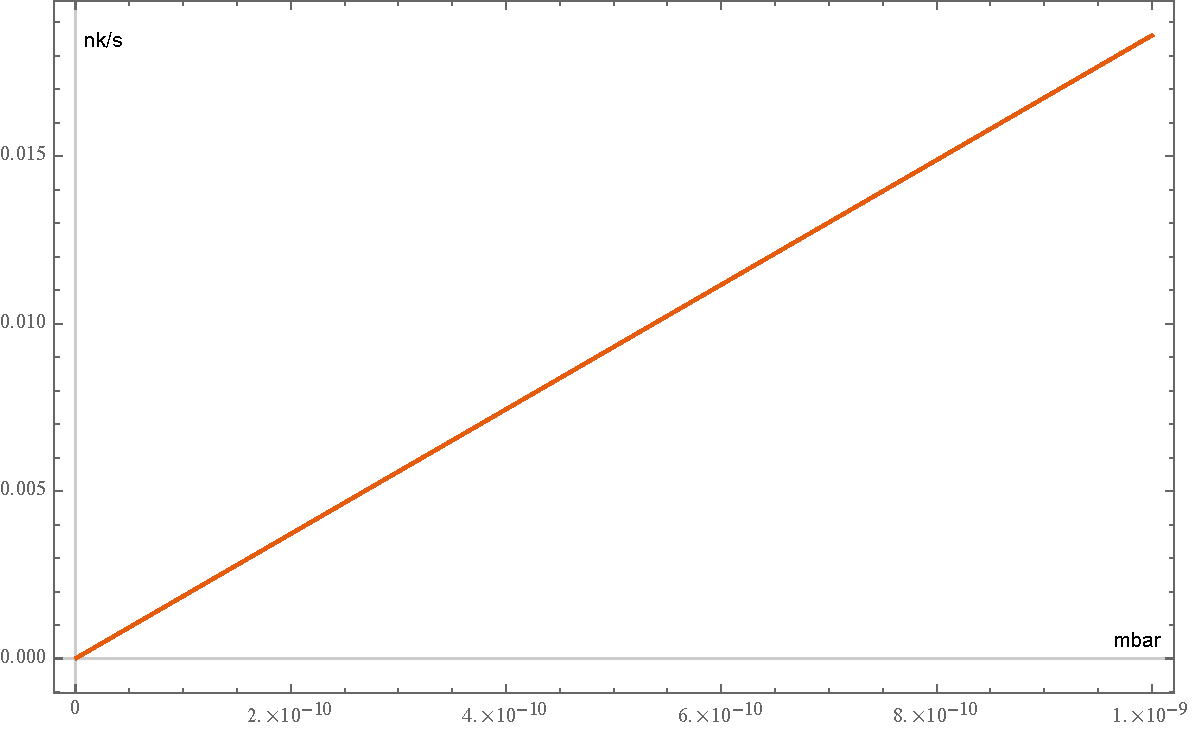
\includegraphics[width=1\textwidth]{heatingrate}
\caption{Pressure Vs heating rate}
\label{fig:heating rate}
\end{figure}

目前在我们的十一通腔体中,真空度在$8*10^{-10} mbar$,根据以上公式,可以计算出加热率为0.015 nK/s,非常小,几乎可以忽略。这也说明了在$10^{-10} mbar$真空下背景气体对于BEC原子团的加热效应比较小。

我们可以计算出导致加热的碰撞占总碰撞的比例为

\begin{equation}
\frac{E_h}{7E_c}=\frac{9*200 nK }{7*43 mK}=5.98*10^{-6}
\end{equation}

可见这部分比例是非常少的,大部分碰撞都导致了BEC原子团原子数的减少。如果按照上面的碰撞率来算,在$8*10^{-10} mbar$,真空度下,经过0.1s,BEC就不存在了。这个碰撞率的估算比较粗略,考虑到BEC的密度有限,实际情况下碰撞率并不会那么高,我们的真空度比一般BEC实验要求的真空度高两个量级以上,可以估算BEC的寿命要低两个量级,所以1s左右的存活状态是可能有的。


%\section{参考文献}
%%%%%%%%%%%%%%%%%%%%%%%%%%%%%%%%%%%%%%%%%%%%%%%%%%%%%%%%%%%%%%%%
%  参考文献
%%%%%%%%%%%%%%%%%%%%%%%%%%%%%%%%%%%%%%%%%%%%%%%%%%%%%%%%%%%%%%%%
\small
\begin{thebibliography}{99}
\setlength{\itemsep}{0pt}
\setlength{\parskip}{0pt}  %段落之间的竖直距离
\bibitem{mc1} M. Inguscio, S. Stringari, Carl Edwin Wieman, Società italiana di fisica. Bose-Einstein Condensation in Atomic Gases: Proceedings of the International School of Physics "Enrico Fermi", Varenna on Lake Como, Villa Monastero, 7-17 July 1998

\end{thebibliography}

\end{document}

